% Options for packages loaded elsewhere
\PassOptionsToPackage{unicode}{hyperref}
\PassOptionsToPackage{hyphens}{url}
%
\documentclass[
  12pt,
  letterpaper,
]{article}
\usepackage{amsmath,amssymb}
\usepackage{lmodern}
\usepackage{iftex}
\ifPDFTeX
  \usepackage[T1]{fontenc}
  \usepackage[utf8]{inputenc}
  \usepackage{textcomp} % provide euro and other symbols
\else % if luatex or xetex
  \usepackage{unicode-math}
  \defaultfontfeatures{Scale=MatchLowercase}
  \defaultfontfeatures[\rmfamily]{Ligatures=TeX,Scale=1}
\fi
% Use upquote if available, for straight quotes in verbatim environments
\IfFileExists{upquote.sty}{\usepackage{upquote}}{}
\IfFileExists{microtype.sty}{% use microtype if available
  \usepackage[]{microtype}
  \UseMicrotypeSet[protrusion]{basicmath} % disable protrusion for tt fonts
}{}
\makeatletter
\@ifundefined{KOMAClassName}{% if non-KOMA class
  \IfFileExists{parskip.sty}{%
    \usepackage{parskip}
  }{% else
    \setlength{\parindent}{0pt}
    \setlength{\parskip}{6pt plus 2pt minus 1pt}}
}{% if KOMA class
  \KOMAoptions{parskip=half}}
\makeatother
\usepackage{xcolor}
\usepackage[margin = 1in]{geometry}
\usepackage{color}
\usepackage{fancyvrb}
\newcommand{\VerbBar}{|}
\newcommand{\VERB}{\Verb[commandchars=\\\{\}]}
\DefineVerbatimEnvironment{Highlighting}{Verbatim}{commandchars=\\\{\}}
% Add ',fontsize=\small' for more characters per line
\usepackage{framed}
\definecolor{shadecolor}{RGB}{248,248,248}
\newenvironment{Shaded}{\begin{snugshade}}{\end{snugshade}}
\newcommand{\AlertTok}[1]{\textcolor[rgb]{0.94,0.16,0.16}{#1}}
\newcommand{\AnnotationTok}[1]{\textcolor[rgb]{0.56,0.35,0.01}{\textbf{\textit{#1}}}}
\newcommand{\AttributeTok}[1]{\textcolor[rgb]{0.77,0.63,0.00}{#1}}
\newcommand{\BaseNTok}[1]{\textcolor[rgb]{0.00,0.00,0.81}{#1}}
\newcommand{\BuiltInTok}[1]{#1}
\newcommand{\CharTok}[1]{\textcolor[rgb]{0.31,0.60,0.02}{#1}}
\newcommand{\CommentTok}[1]{\textcolor[rgb]{0.56,0.35,0.01}{\textit{#1}}}
\newcommand{\CommentVarTok}[1]{\textcolor[rgb]{0.56,0.35,0.01}{\textbf{\textit{#1}}}}
\newcommand{\ConstantTok}[1]{\textcolor[rgb]{0.00,0.00,0.00}{#1}}
\newcommand{\ControlFlowTok}[1]{\textcolor[rgb]{0.13,0.29,0.53}{\textbf{#1}}}
\newcommand{\DataTypeTok}[1]{\textcolor[rgb]{0.13,0.29,0.53}{#1}}
\newcommand{\DecValTok}[1]{\textcolor[rgb]{0.00,0.00,0.81}{#1}}
\newcommand{\DocumentationTok}[1]{\textcolor[rgb]{0.56,0.35,0.01}{\textbf{\textit{#1}}}}
\newcommand{\ErrorTok}[1]{\textcolor[rgb]{0.64,0.00,0.00}{\textbf{#1}}}
\newcommand{\ExtensionTok}[1]{#1}
\newcommand{\FloatTok}[1]{\textcolor[rgb]{0.00,0.00,0.81}{#1}}
\newcommand{\FunctionTok}[1]{\textcolor[rgb]{0.00,0.00,0.00}{#1}}
\newcommand{\ImportTok}[1]{#1}
\newcommand{\InformationTok}[1]{\textcolor[rgb]{0.56,0.35,0.01}{\textbf{\textit{#1}}}}
\newcommand{\KeywordTok}[1]{\textcolor[rgb]{0.13,0.29,0.53}{\textbf{#1}}}
\newcommand{\NormalTok}[1]{#1}
\newcommand{\OperatorTok}[1]{\textcolor[rgb]{0.81,0.36,0.00}{\textbf{#1}}}
\newcommand{\OtherTok}[1]{\textcolor[rgb]{0.56,0.35,0.01}{#1}}
\newcommand{\PreprocessorTok}[1]{\textcolor[rgb]{0.56,0.35,0.01}{\textit{#1}}}
\newcommand{\RegionMarkerTok}[1]{#1}
\newcommand{\SpecialCharTok}[1]{\textcolor[rgb]{0.00,0.00,0.00}{#1}}
\newcommand{\SpecialStringTok}[1]{\textcolor[rgb]{0.31,0.60,0.02}{#1}}
\newcommand{\StringTok}[1]{\textcolor[rgb]{0.31,0.60,0.02}{#1}}
\newcommand{\VariableTok}[1]{\textcolor[rgb]{0.00,0.00,0.00}{#1}}
\newcommand{\VerbatimStringTok}[1]{\textcolor[rgb]{0.31,0.60,0.02}{#1}}
\newcommand{\WarningTok}[1]{\textcolor[rgb]{0.56,0.35,0.01}{\textbf{\textit{#1}}}}
\usepackage{longtable,booktabs,array}
\usepackage{calc} % for calculating minipage widths
% Correct order of tables after \paragraph or \subparagraph
\usepackage{etoolbox}
\makeatletter
\patchcmd\longtable{\par}{\if@noskipsec\mbox{}\fi\par}{}{}
\makeatother
% Allow footnotes in longtable head/foot
\IfFileExists{footnotehyper.sty}{\usepackage{footnotehyper}}{\usepackage{footnote}}
\makesavenoteenv{longtable}
\usepackage{graphicx}
\makeatletter
\def\maxwidth{\ifdim\Gin@nat@width>\linewidth\linewidth\else\Gin@nat@width\fi}
\def\maxheight{\ifdim\Gin@nat@height>\textheight\textheight\else\Gin@nat@height\fi}
\makeatother
% Scale images if necessary, so that they will not overflow the page
% margins by default, and it is still possible to overwrite the defaults
% using explicit options in \includegraphics[width, height, ...]{}
\setkeys{Gin}{width=\maxwidth,height=\maxheight,keepaspectratio}
% Set default figure placement to htbp
\makeatletter
\def\fps@figure{htbp}
\makeatother
\setlength{\emergencystretch}{3em} % prevent overfull lines
\providecommand{\tightlist}{%
  \setlength{\itemsep}{0pt}\setlength{\parskip}{0pt}}
\setcounter{secnumdepth}{5}
\usepackage{longtable}
\usepackage[utf8]{inputenc}
\usepackage[spanish]{babel}\decimalpoint
\setlength{\parindent}{1.25cm}
\usepackage{amsmath}
\usepackage{xcolor}
\usepackage{cancel}
\usepackage{array}
\usepackage{float}
\usepackage{multirow}
\usepackage{booktabs}
\usepackage{longtable}
\usepackage{array}
\usepackage{multirow}
\usepackage{wrapfig}
\usepackage{float}
\usepackage{colortbl}
\usepackage{pdflscape}
\usepackage{tabu}
\usepackage{threeparttable}
\usepackage{threeparttablex}
\usepackage[normalem]{ulem}
\usepackage{makecell}
\usepackage{xcolor}
\ifLuaTeX
  \usepackage{selnolig}  % disable illegal ligatures
\fi
\IfFileExists{bookmark.sty}{\usepackage{bookmark}}{\usepackage{hyperref}}
\IfFileExists{xurl.sty}{\usepackage{xurl}}{} % add URL line breaks if available
\urlstyle{same} % disable monospaced font for URLs
\hypersetup{
  hidelinks,
  pdfcreator={LaTeX via pandoc}}

\author{}
\date{\vspace{-2.5em}}

\begin{document}

\begin{titlepage}
   \Large{
   \begin{center}
       \vspace*{1cm}

       \textbf{Tarea 1}

            
       \vspace{1.1cm}
       
       Estudiantes
       
       \vspace{0.5cm}
        
	\textbf{Jhonatan Smith Garcia Muñoz}        

       \textbf{Diego Cano} \\

	\textbf{Juan Manuel Sanchez} \\

	\textbf{}

              \vspace{1cm}
       
       Docente
       
       \vspace{0.5cm}

       \textbf{Juan Carlos Salazar Uribe}
       
       \vspace{0.4cm}

       \vspace{1.4cm}
       
       Asignatura
       
       \vspace{0.5cm}

       \textbf{Introdución al analisís de supervivencia}

       \vfill

            
       \vspace{0.4cm}
     
       
\includegraphics[width=0.4\textwidth]{logounal.png}
            
       Sede Medellín\\
       17 de marzo de 2023
       
   \end{center}
   }
\end{titlepage}
\thispagestyle{empty}
\tableofcontents
\newpage

\pagestyle{myheadings}
\setcounter{page}{4}

\section{Ejercicio 1}

En las siguientes situaciones identifique: el evento de interes y la
variable respuesta.

\textbf{Solucion}

\emph{a)} Se realiza un seguimiento durante 13 años a un grupo de
adultos de al menos 60 años de edad para ver que tanto tiempo permanecen
vivos.

\begin{itemize}
\item
  Evento de interes: Fallecimiento
\item
  Variable respuesta: Tiempo de supervivencia en años para los adultos
  de al menos 60 años de edad
\end{itemize}

\emph{b)} Un grupo de pacientes con un trasplante de corazon son
monitoreados para ver cuanto tiempo sobreviven

\begin{itemize}
\item
  Evento de interes: La muerte
\item
  Tiempo de supervivecia para pacientes que han sido sometidos a
  transplante de corazon.
\end{itemize}

\section{Ejercicio 2}

Resuelva a MANO, usando los datos sobre Hepatitis Crónica Activa (CAH).
Estos datos son de un ensayo clinico descrito en Kirk (1980). 44
pacientes con CAH se aleatorizaron a una droga llamada prednisolona o a
un grupo de control sin tratamiento. El tiempo de supervivenvia en
meses, despues de ser admitido al ensayo es la variables respuesta. Con
estos datos obtenga una estimación de KM y el de NA. Note que debe
evidenciar tablas de vida. No olvide el analisis descriptivo. Interprete

\textbf{Solucion}

A continuacion se muestra ña estructura general de la base de datos.
Tenga presente que se tienen ensayos clinicos para 44 pacientes, donde
existen dos grupos: Control con tratamiento y control sin tratamiento. 1
Representa fallas y 0 representa las censuras. Se presentan los primeros
6 datos de la tabla de manera ilustrativa.

\begin{verbatim}
## 
## -- Column specification --------------------------------------------------------
## cols(
##   id = col_double(),
##   group = col_double(),
##   time = col_double(),
##   status = col_double()
## )
\end{verbatim}

\begin{verbatim}
## Warning: 1 parsing failure.
## row col  expected    actual                                                                               file
##  23  -- 4 columns 5 columns 'C:/Users/jhsga/OneDrive/Escritorio/GitHub/Asignaturas-UNAL/SUPERVIVENCIA/CAH.txt'
\end{verbatim}

\begin{tabular}{r|r|r|r}
\hline
id & group & time & status\\
\hline
1 & 1 & 2 & 1\\
\hline
2 & 1 & 2 & 1\\
\hline
3 & 1 & 12 & 1\\
\hline
4 & 1 & 54 & 1\\
\hline
5 & 1 & 56 & 0\\
\hline
6 & 1 & 68 & 1\\
\hline
\end{tabular}

Esta informacion puede ser resumida de la siguiente manera:

Tabla 1: Tabla de vida grupo 1

\begin{longtable}[]{@{}rccr@{}}
\toprule()
\(t_j\) & \(d_j\) & \(q_j\) & \(n_j\) \\
\midrule()
\endhead
\(t_0\)=0 & 0 & 0 & 22(22 unidades sobreviven \textgreater= 0 meses ) \\
\(t_1\)=2 & 2 & 0 & 22(22 unidades sobreviven \textgreater= 2 meses ) \\
\(t_2\)=12 & 1 & 0 & 20(20 unidades sobreviven \textgreater= 12 meses
) \\
\(t_3\)=54 & 1 & 1 & 19(19 unidades sobreviven \textgreater= 54 meses
) \\
\(t_4\)=68 & 1 & 0 & 17(17 unidades sobreviven \textgreater= 68 meses
) \\
\(t_5\)=89 & 1 & 0 & 16(16 unidades sobreviven \textgreater= 89 meses
) \\
\(t_6\)=96 & 2 & 5 & 15(15 unidades sobreviven \textgreater= 96 meses
) \\
\(t_7\)=143 & 1 & 1 & 8(8 unidades sobreviven \textgreater= 143 meses
) \\
\(t_8\)=146 & 1 & 2 & 6(6 unidades sobreviven \textgreater= 146 meses
) \\
\(t_9\)=168 & 1 & 2 & 3(3 unidades sobreviven \textgreater= 168 meses
) \\
TOTAL & 11 & 11 & 11+11=22 \\
\bottomrule()
\end{longtable}

Con esto, es necesario analizar el tiempo promedio \(\hat{T}\) y el
Hazar \(\hat{h}\) para el grupo 1 que se define respectivamente como:

\[
\bar{T}=\frac{1}{n} \sum_{i=1}^n t_i
\]

\[
\bar{T}=\frac{1}{22} \sum_{i=1}^{22} t_i=109.3636
\]

\[
\bar{h}=\frac{11}{22(109.3636)}=0.004571905
\]

Tabla 2: Tabla de vida Grupo 2

\begin{longtable}[]{@{}rllr@{}}
\toprule()
\(t_j\) & \(d_j\) & \(q_j\) & \(n_j\) \\
\midrule()
\endhead
\(t_0\)=0 & 0 & 0 & 22(22 unidades sobreviven \textgreater= 0 meses) \\
\(t_1\)=2 & 1 & 0 & 22(22 unidades sobreviven \textgreater= 2 meses ) \\
\(t_2\)=3 & 1 & 0 & 21 (21 unidades sobreviven \textgreater= 3 meses) \\
\(t_3\)=4 & 1 & 0 & 20(20 unidades sobreviven \textgreater= 4 meses ) \\
\(t_4\)=7 & 1 & 0 & 19(19 unidades sobreviven \textgreater= 7 meses ) \\
\(t_5\)=10 & 1 & 0 & 18(18 unidades sobreviven \textgreater= 10
meses) \\
\(t_6\)=22 & 1 & 0 & 17(17 unidades sobreviven \textgreater= 22 meses
) \\
\(t_7\)=28 & 1 & 0 & 16(16 unidades sobreviven \textgreater= 28 meses
) \\
\(t_8\)=29 & 1 & 0 & 15(15 unidades sobreviven \textgreater= 29 meses
) \\
\(t_9\)=32 & 1 & 0 & 14(14 unidades sobreviven \textgreater= 32
meses) \\
\(t_10\)=37 & 1 & 0 & 13(13 unidades sobreviven \textgreater= 37 meses
) \\
\(t_11\)=40 & 1 & 0 & 12(12 unidades sobreviven \textgreater= 40 meses
) \\
\(t_12\)=41 & 1 & 0 & 11(11 unidades sobreviven \textgreater= 41
meses) \\
\(t_13\)=54 & 1 & 0 & 10(10 unidades sobreviven \textgreater= 54 meses
) \\
\(t_14\)=61 & 1 & 0 & 9 (9 unidades sobreviven \textgreater= 61 meses
) \\
\(t_15\)=63 & 1 & 0 & 8(8 unidades sobreviven \textgreater= 63 meses) \\
\(t_16\)=71 & 1 & 6 & 7 unidades sobreviven \textgreater= 71 meses ) \\
TOTAL & 16 & 6 & 16+6=22 \\
\bottomrule()
\end{longtable}

Ahora para el grupo 2, tl tiempo promedio \(\hat{T}\) y \(\hat{h}\) es:

\[
\bar{T}=\frac{1}{n} \sum_{i=1}^n t_i
\]

\[
\bar{T}=\frac{1}{22} \sum_{i=1}^{22} t_i=64.72727
\]

\[
\bar{h}=\frac{11}{22(109.3636)}=0.007724719
\]

A mayor Hazard es menor la probabilidad de supervivencia (Evidentemente,
por eso el nombre), en este casi, se ve claramente que
\(\hat{h_1}<\hat{h_2}\) y a su vez; \(\hat{T_1}>\hat{T_2}\). Basado en
esto, se podria concluir que la supervivencia del grupo 2 es menor que
la del grupo 1. Esto podria evidenciarse en el siguiente analisis
grafico.

\begin{Shaded}
\begin{Highlighting}[]
\NormalTok{df}\SpecialCharTok{$}\NormalTok{group }\OtherTok{=}\NormalTok{ df}\SpecialCharTok{$}\NormalTok{group }\SpecialCharTok{\%\textgreater{}\%} \FunctionTok{as.factor}\NormalTok{()}
\FunctionTok{ggplot}\NormalTok{(df, }\FunctionTok{aes}\NormalTok{(}\AttributeTok{x =}\NormalTok{ group, }\AttributeTok{y =}\NormalTok{ time, }\AttributeTok{group =}\NormalTok{ group, }\AttributeTok{fill =}\NormalTok{ group)) }\SpecialCharTok{+}
  \FunctionTok{geom\_boxplot}\NormalTok{( }\AttributeTok{color =} \StringTok{"\#404040"}\NormalTok{)}\SpecialCharTok{+}
  \FunctionTok{stat\_summary}\NormalTok{(}\AttributeTok{fun =}\NormalTok{ mean, }\AttributeTok{geom =} \StringTok{"point"}\NormalTok{, }\AttributeTok{shape =} \DecValTok{20}\NormalTok{,}
               \AttributeTok{size =} \DecValTok{3}\NormalTok{, }\AttributeTok{color =} \StringTok{"red"}\NormalTok{,}\AttributeTok{position =} \FunctionTok{position\_dodge}\NormalTok{(}\AttributeTok{width =} \FloatTok{0.75}\NormalTok{))}\SpecialCharTok{+}
  \FunctionTok{labs}\NormalTok{(}\AttributeTok{title =} \StringTok{"Tiempo de respuesta por grupo"}\NormalTok{, }
       \AttributeTok{x =} \StringTok{"Grupo"}\NormalTok{, }
       \AttributeTok{y =} \StringTok{"Tiempo"}\NormalTok{) }\SpecialCharTok{+}
  \FunctionTok{theme\_bw}\NormalTok{()}
\end{Highlighting}
\end{Shaded}

\begin{center}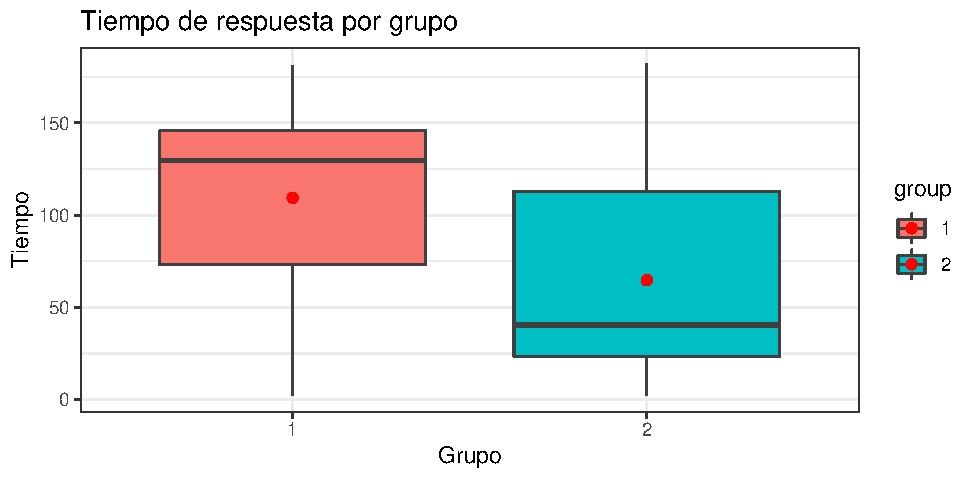
\includegraphics{Trabajo-1-Supervivencia_files/figure-latex/unnamed-chunk-2-1} \end{center}

Note que claramente las medias de ambos procesos (puntos rojos) se
encuentran uno por encima de la otra. Esto da un indicio que los
individuos del grupo 1 en comparación a los individuos del grupo 2
presentan un tiempo de supervivencia promedio mayor.

En el grupo 1 el 50\% de los datos esta aproximadamente por encima de
120 meses y el 50\% por debajo, mientras que en el grupo 2 el 50\% esta
aproximadamente por encima de 40 meses y el 50\% por debajo, es decir,
que se presenta una diferencia significativa en el promedio de los
tiempos hasta que el individuo falla entre el grupo 1 y el grupo 2

Dado esto, se procede a realizar entonces las estimaciones con KM
(Kaplan-Meier):

\hypertarget{estimacion-de-km-para-grupo-1}{%
\subsection{Estimacion de KM para grupo
1}\label{estimacion-de-km-para-grupo-1}}

\[
\begin{array}{|r|l|r|r|l|}
t_{(j)} & d_j & q_j & n_j & \hat{S}_{K M}\left(t_j\right) \\
\hline 0 & 0 & 0 & 22 & 1-\frac{0}{22}=1 \\
2 & 2 & 0 & 22 & 1 \mathrm{x}\left(1-\frac{2}{22}\right)=\frac{10}{11} \approx 0.9091 \\
12 & 1 & 0 & 20 & \frac{10}{11} \mathrm{x}\left(1-\frac{1}{20}\right)=\frac{19}{22} \approx 0.8636 \\
54 & 1 & 1 & 19 & \frac{19}{22} \mathrm{x}\left(1-\frac{1}{19}\right)=\frac{9}{11} \approx 0.8182 \\
68 & 1 & 0 & 17 & \frac{9}{11} \mathrm{x}\left(1-\frac{1}{17}\right)=\frac{144}{187} \approx 0.7701 \\
89 & 1 & 0 & 16 & \frac{144}{187} \mathrm{x}\left(1-\frac{1}{16}\right)=\frac{135}{187} \approx 0.7221 \\
96 & 2 & 5 & 15 & \frac{135}{187} \mathrm{x}\left(1-\frac{2}{15}\right)=\frac{117}{187} \approx 0.6257 \\
143 & 1 & 1 & 8 & \frac{117}{187} \mathrm{x}\left(1-\frac{1}{8}\right)=\frac{819}{146} \approx 0.5475 \\
146 & 1 & 2 & 6 & \frac{819}{1496} \mathrm{x}\left(1-\frac{1}{6}\right)=\frac{1365}{2992} \approx 0.4562 \\
168 & 1 & 2 & 3 & \frac{1365}{2992} \mathrm{x}\left(1-\frac{1}{3}\right)=\frac{455}{1496} \approx 0.3041 \\
\hline
\end{array}
\] \#\# Estimacion de KM para el grupo 2

\[
\begin{array}{|r|l|r|r|l|}
t_{(j)} & d_j & q_j & n_j & \hat{S}_{K M}\left(t_j\right) \\
\hline 0 & 0 & 0 & 22 & 1-\frac{0}{22}=1 \\
2 & 1 & 0 & 22 & 1 \mathrm{x}\left(1-\frac{1}{22}\right)=\frac{21}{22} \approx 0.9545 \\
3 & 1 & 0 & 21 & \frac{21}{22} \mathrm{x}\left(1-\frac{1}{21}\right)=\frac{10}{11} \approx 0.9091 \\
4 & 1 & 0 & 20 & \frac{10}{11} \mathrm{x}\left(1-\frac{1}{20}\right)=\frac{19}{22} \approx 0.8636 \\
7 & 1 & 0 & 19 & \frac{19}{22} \mathrm{x}\left(1-\frac{1}{19}\right)=\frac{9}{11} \approx 0.8182 \\
10 & 1 & 0 & 18 & \frac{9}{11} \mathrm{x}\left(1-\frac{1}{18}\right)=\frac{17}{22} \approx 0.7727 \\
22 & 1 & 0 & 17 & \frac{17}{22} \mathrm{x}\left(1-\frac{1}{17}\right)=\frac{8}{11} \approx 0.7273 \\
28 & 1 & 0 & 16 & \frac{8}{11} \mathrm{x}\left(1-\frac{1}{16}\right)=\frac{15}{22} \approx 0.6818 \\
29 & 1 & 0 & 15 & \frac{15}{22} \mathrm{x}\left(1-\frac{1}{15}\right)=\frac{7}{11} \approx 0.6364 \\
32 & 1 & 0 & 14 & \frac{7}{11} \mathrm{x}\left(1-\frac{1}{14}\right)=\frac{13}{22} \approx 0.5909 \\
37 & 1 & 0 & 13 & \frac{13}{22} \mathrm{x}\left(1-\frac{1}{13}\right)=\frac{6}{11} \approx 0.5455 \\
40 & 1 & 0 & 12 & \frac{6}{11} \mathrm{x}\left(1-\frac{1}{12}\right)=\frac{1}{2} \approx 0.5 \\
41 & 1 & 0 & 11 & \frac{1}{2} \mathrm{x}\left(1-\frac{1}{11}\right)=\frac{5}{11} \approx 0.4545 \\
54 & 1 & 0 & 10 & \frac{5}{11} \mathrm{x}\left(1-\frac{1}{10}\right)=\frac{9}{22} \approx 0.4091 \\
61 & 1 & 0 & 9 & \frac{9}{22} \mathrm{x}\left(1-\frac{1}{9}\right)=\frac{4}{11} \approx 0.3636 \\
63 & 1 & 0 & 8 & \frac{4}{11} \mathrm{x}\left(1-\frac{1}{8}\right)=\frac{7}{22} \approx 0.3182 \\
71 & 1 & 6 & 7 & \frac{7}{22} \mathrm{x}\left(1-\frac{1}{7}\right)=\frac{3}{11} \approx 0.2727 \\
\hline
\end{array}
\]

\end{document}
